\documentclass[11pt, a4paper, DIV=12]{scrartcl}

% useful packages 
\usepackage{mathtools}
\usepackage{physics}
\usepackage{graphicx}					  
\graphicspath{{figs/}}



\usepackage{amssymb}
\usepackage{amsmath}
\usepackage{hyperref}
\usepackage[separate-uncertainty=true]{siunitx}
\usepackage{xcolor}
\usepackage{braket} % easy braket notation
\usepackage{enumitem}
\usepackage{booktabs}
\usepackage{here}
\usepackage{cprotect}

\usepackage[backend=biber, sorting=none]{biblatex}
\bibliography{refs.bib}

% \numberwithin{equation}{section}

\title{Simulation of 1-Dimensional Ising Model}
\date{\today}
\author{Harilal Bhattarai \& Marcel}
\begin{document}
	\maketitle
	
\section{Introduction}
The Ising model is a wonderful sandbox to study critical phenomena with numerical methods. It helps to investigate the magnetization in the absence of the external magnetic field.\\

In this report, firstly, We can include some theoretical background on theory part. Secondly, we will try to present the answers the questions of this exercise-sheet-1 in analysis part, also, with illustration of the results of simulation with the help of plots.  

\section{Theory}

This system of spins is immersed in a heat bath of constant temperature T and in an external magnetic field h. Its dynamics are governed by the Hamiltonian,
\begin{equation}
H(s)= -J \sum_{<x,y>}s_{x}s_{y} - h \sum_{x}s_{x}
\end{equation}
$ <x,y> $ denotes the nearest-neighbor pair x and y on the chain, J is a real number and we assume periodic boundary conditions.

In 1d the partition function can be determined analytically as a function of N, J/T, and h/T as,
\begin{equation}
\text{Z}=\lambda^{\text{N}}_{+} + \lambda^{\text{N}}_{-}
\end{equation}
Where, 
\begin{equation}
 \lambda^{\text{N}}_{\pm}= e^{\frac{J}{T}} \bigg(cosh(\frac{h}{T})\pm \sqrt{Sinh(\frac{h}{T})^2 + e^{-4(\frac{J}{T})}} \bigg) 
 \label{Equ:lambda}
	\end{equation}
The magnetization can be determine with the help of Ising model as, 
\begin{equation}
<m> = -\frac{\text{h}}{\text{T}} \frac{\partial\log \text{Z}}{\partial \text{h}}
\label{equ:m}
\end{equation}  

\section{Analysis}
In the partition function total angular momentum, J is the interaction of the spins in a system. It is $ \pm 1 $ for parallel and 0 for 
anti-parallel spins for spin $ \frac{1}{2} $ particles. Also, J= 2 for spin 1 particles. For parallel orientation, potential energy gets reduced compared to anti-parallel arrangement. since Coulomb-repulsion is reduced
due to larger average inter particle distance.\\

To determine the dependency of $ <m> $ on the external field strength h for fixed N and the number of spins N for fixed h. To do so, we have taken the N=20, J=1 and $h \ [-1, 1]$. Here, for analytic solution we used the expression \ref{equ:m} without considering all spin configurations but we can also determined the numerical value by simulation.

To compare these both(numeric and analytic) results, we plotted a graph numbers vs magnetization with change the external magnetic field. from figure \ref{fig:Nconst}, We can see that at h=0 there is no any magnetization; however, if the external field is positive, we also get a positive magnetization. 
\begin{figure}[H]
	\centering
	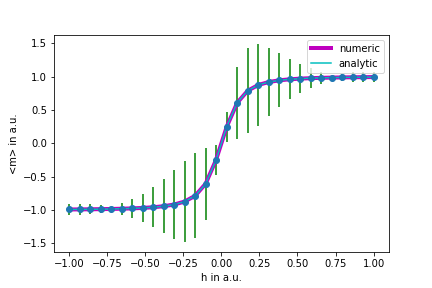
\includegraphics[width=0.8\linewidth]{Nconst.png}
	\caption{The number of spins N for fixed h.}
	\label{fig:Nconst}
\end{figure}


Again, we have plotted a graph number vs magnetization with considering constant external magnetic field. We have chosen h= 0.5. Also, we can compare these analytic and numerical data. From figure \ref{fig:hconst} we can see that change N. but since we are looking for the magnetization per spin. we expect that it does not change with higher N and this is the case
   \begin{figure}[H]
   	\centering
   	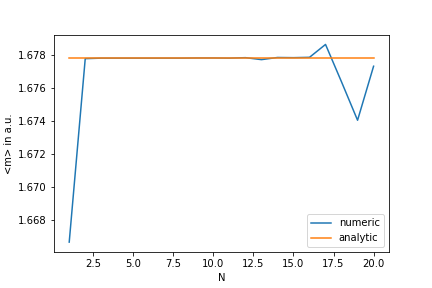
\includegraphics[width=0.8\linewidth]{hconst.png}
   	\caption{The external field strength h for fixed N.}
   	\label{fig:hconst}
   \end{figure}
\section{conclusion}

\begin{thebibliography}{12}
\bibitem{exercise-sheet} 
	Unknown, Exercise-sheet, 2020.
		
\bibitem{wiki} 
	Satya pal singh, \textit{The Ising Model: Brief Introduction and Its Application}, 2020.
	
\end{thebibliography}

\end{document}
